\de{ĐỀ THI GIỮA HỌC KỲ I NĂM HỌC 2023-2024}{THPT Tây Thạnh}
\begin{bt}%[0D3H1-2]%[Dự án đề kiểm tra Toán 10 GHKI NH23-24- Huỳnh Quy]%[THPT Tây Thạnh]
	Tìm tập xác định của hàm số $y=f(x)=\dfrac{\sqrt{2x+9}+5x}{x+4}$.
	\loigiai{
		Hàm số xác định $\Leftrightarrow \heva{&x+4\ne 0\\&2x+9\geq 0}\Leftrightarrow\heva{&x\ne -4\\&x\geq -\dfrac{9}{2}}$.\\
		Vậy tập xác định là $D=\left[-\dfrac{9}{2};+\infty\right)\setminus\{-4\}$.
	}
\end{bt}

\begin{bt}%[0D3H1-5]%[Dự án đề kiểm tra Toán 10 GHKI NH23-24- Huỳnh Quy]%[THPT Tây Thạnh]
	Tìm khoảng đồng biến, nghịch biến của hàm số có đồ thị như hình sau:
	\begin{center}
		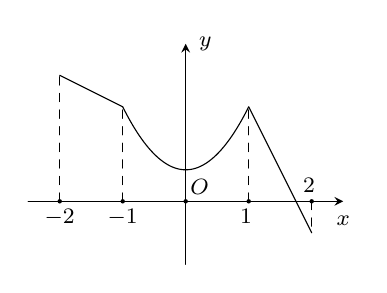
\begin{tikzpicture}[font=\footnotesize,line join=round, line cap=round, >=stealth,scale=0.8] 
			\def \xmin{-2.5}\def \xmax{2.5}\def \ymin{-1}\def \ymax{2.5} 
			\draw[->] (\xmin,0)--(\xmax,0) node[shift=(-90:0.25)] {$x$};
			\draw[->] (0,\ymin)--(0,\ymax) node[shift=(0:0.25)] {$y$};
			\fill (0,0) circle(1pt) node[shift=(45:0.25)]{$O$}
			(1,0) circle(1pt) node[shift=(-100:0.2)]{$1$}
			(2,0) circle(1pt) node[shift=(100:0.2)]{$2$}
			(-2,0) circle(1pt) node[shift=(-90:0.2)]{$-2$}
			(-1,0) circle(1pt) node[shift=(-90:0.2)]{$-1$}
			;
			\draw (-2,2)--(-1,1.5) (1,1.5)--(2,-0.5);
			\begin{scope}
				\clip (\xmin,\ymin) rectangle (\xmax,\ymax); 
				\draw[smooth,samples=100,domain=-1:1] plot(\x,{(\x)^2+0.5});
				%			\draw[smooth,samples=100,domain=\xmin:\xmax] plot(\x,{4-\x});
			\end{scope}
			\draw[dashed] (-2,0)--(-2,2) (-1,0)--(-1,1.5) (1,0)--(1,1.5) (2,0)--(2,-0.5);
		\end{tikzpicture}
	\end{center}
	\loigiai{
		Ta thấy trên các khoảng $(-2;0)$ và $(1;2)$ đồ thị hàm số đi xuống từ trái sang phải nên nghịch biến.\\
		Trên khoảng $(0;1)$, đồ thị hàm số đi lên từ trái sang phải nên hàm số đồng biến.
	}
\end{bt}
\begin{bt}%[0D3H2-3]%[Dự án đề kiểm tra Toán 10 GHKI NH23-24- Huỳnh Quy]%[THPT Tây Thạnh]
	Hãy tìm tập xác định, tọa độ đỉnh, trục đối xứng và vẽ đồ thị hàm số $y=x^2-4x+2$.
	\loigiai{
		Tập xác định là $\mathscr{D}=\mathbb{R}$.\\
		Tọa độ đỉnh $I\left(2;-2\right)$.\\
		Trục đối xứng là đường thẳng $x=-2$.\\
		Hệ số $a=1>0$ nên bề lõm quay lên.\\
		Bảng giá trị:
		\begin{center}
			\begin{tabular}{|c|c|c|c|c|c|}\hline
				{$x$}&{$0$}&{$1$}&{$2$}&{$3$}&{$4$}\\\hline
				{$y$}&{$2$}&{$-1$}&{$-2$}&{$-1$}&{$2$}\\\hline	
			\end{tabular}	
		\end{center}
		Đồ thị:
		\begin{center}
			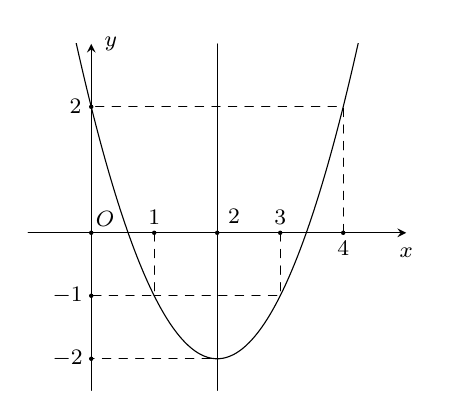
\begin{tikzpicture}[font=\footnotesize,line join=round, line cap=round, >=stealth,scale=0.8] 
				\def \xmin{-1}\def \xmax{5}\def \ymin{-2.5}\def \ymax{3} 
				\draw[->] (\xmin,0)--(\xmax,0) node[shift=(-90:0.25)] {$x$};
				\draw[->] (0,\ymin)--(0,\ymax) node[shift=(0:0.25)] {$y$};
				\fill (0,0) circle(1pt) node[shift=(45:0.25)]{$O$}
				(1,0) circle(1pt) node[shift=(90:0.2)]{$1$}
				(2,0) circle(1pt) node[shift=(45:0.3)]{$2$}
				(3,0) circle(1pt) node[shift=(90:0.2)]{$3$}
				(4,0) circle(1pt) node[shift=(-90:0.2)]{$4$}
				(0,2) circle(1pt) node[shift=(180:0.2)]{$2$}
				(0,-2) circle(1pt) node[shift=(180:0.3)]{$-2$}
				(0,-1) circle(1pt) node[shift=(180:0.3)]{$-1$};
				\begin{scope}
					\clip (\xmin,\ymin) rectangle (\xmax,\ymax); 
					\draw[smooth,samples=100,domain=\xmin:\xmax] plot(\x,{(\x)^2-4*(\x)+2});
				\end{scope}
				\draw[dashed] (1,0)--(1,-1)--(0,-1) (2,0)--(2,-2)--(0,-2) (3,0)--(3,-1)--(1,-1) (4,0)--(4,2)--(0,2);
				\draw (2,\ymax)--(2,\ymin);
			\end{tikzpicture}
		\end{center}
	}
\end{bt}
%Câu 1...........................
\begin{bt}%[0H4H2-2]%[Dự án đề kiểm tra Toán 11 GHKI NH23-24- Quang Vinh NT]%[THPT - Tp HCM]
	Cho tam giác $ABC$ có $AC=\sqrt{17}$, $AB=7$, $\cos A=\dfrac{\sqrt{17}}{17}$.
	\begin{enumerate}
		\item  Tính độ dài cạnh $BC$, bán kính đường tròn ngoại tiếp, chiều cao kẻ từ đỉnh $C$ của tam giác $ABC$.
		\item Gọi $N$ là chân đường cao hạ từ đỉnh $C$ và điểm $L$ trên cạnh $BC$ sao cho $CL=2LB$. Tính diện tích tam giác $CLN$. \\
		\textbf{(Lưu ý: các số liệu trong câu phải được tính bằng số đúng.)}
	\end{enumerate}
	\loigiai{
		\begin{center}
			\begin{tikzpicture}[scale=1, font=\footnotesize, line join=round, line cap=round, >=stealth] 
				\path (0,0) coordinate (B)
				--++(6,0) coordinate (A)
				--++ (-2,3) coordinate (C)
				($(B)!(C)!(A)$) coordinate (N)
				(C)--(B) coordinate[pos=2/3](L)
				;		
				\draw pic[draw, angle eccentricity=1.5,angle radius = 0.3cm] {right angle = C--N--A}; 
				\draw (A)--(B)--(C)--cycle (C)--(N) (L)--(N);
				\foreach \x/\i in {A/0,B/180,C/90,N/-90,L/150}{
					\path ($(\x)+(\i:3mm)$) node{$\x$};
					\fill[black] (\x) circle (1pt);
				}
			\end{tikzpicture}	
		\end{center}
		\begin{enumerate}	
			\item  Ta có 
			$$BC=\sqrt{AB^2+AC^2-2AB\cdot AC\cdot \cos A}=\sqrt{49+17-2\cdot 7 \cdot \sqrt{17}\cdot \dfrac{\sqrt{17}}{17} }= 2\sqrt{13}.$$
			Và $p=\dfrac{7+\sqrt{17}+2\sqrt{13}}{2}$ nên
			$S_{\triangle ABC}=\sqrt{p(p-\sqrt{17})(p-7)(p-2\sqrt{13})}=14.$\\
			Mà
			$S_{\triangle ABC}=\dfrac{abc}{4R}\Rightarrow R=\dfrac{abc}{4S}=\dfrac{\sqrt{17}\cdot 7 \cdot 2\sqrt{13}}{4\cdot 14}=\dfrac{\sqrt{221}}{4}$.\\
			Ta có $S_{\triangle ABC}=\dfrac{1}{2}\cdot CN\cdot AB\Rightarrow CN = \dfrac{2S_{\triangle ABC}}{AB}=\dfrac{2\cdot 14}{7}= 4$.\\
			\item Xét tam giác $CNB$ vuông tại $N$, ta có
			$$BN=\sqrt{BC^2-CN^2}=\sqrt{52-16}=6.$$
			Do đó 
			\begin{eqnarray*}
				S_{\triangle CLN}&=& \dfrac{1}{2}\cdot CL \cdot CN \sin \widehat{LCN}\\
				&= & \dfrac{1}{2}\cdot \dfrac{2}{3}\cdot CB \cdot CN \sin \widehat{LCN}\\
				&= & \dfrac{2}{3}\cdot S_{\triangle CBN}\\
				&= & \dfrac{2}{3} \cdot \dfrac{1}{2}\cdot CN \cdot BN\\
				&= & \dfrac{1}{3} \cdot 4\cdot 6 = 8.
			\end{eqnarray*}
		\end{enumerate}
	}
\end{bt}

\begin{bt}%[0H4H2-1]%[Dự án đề kiểm tra Toán 11 GHKI NH23-24- Quang Vinh NT]%[THPT - Tp HCM]
	Cho tam giác $ABC$ với bán kính đường tròn ngoại tiếp $R$ và nữa chu vi $p$. Hãy chứng minh rằng: $\sin A+\sin B=\dfrac{1}{R}\left(p-\dfrac{c}{2}\right)$.
	\loigiai{	
		Theo định lý sin:
		$$\dfrac{a}{\sin A}=\dfrac{b}{\sin B}=\dfrac{c}{\sin C}=2R\Rightarrow \heva{&\sin A = \dfrac{a}{2R}\\& \sin B = \dfrac{b}{2R}.}$$
		Nên 
		\begin{eqnarray*}
			\sin A+\sin B	&= & \dfrac{a}{2R}+\dfrac{b}{2R}\\
			&= & \dfrac{a+b}{2R}\\
			&= & \dfrac{a+b+c-c}{2R}\\
			&= & \dfrac{1}{R}\left(\dfrac{a+b+c}{2}-\dfrac{c}{2}\right)\\
			&= & \dfrac{1}{R}\left(p-\dfrac{c}{2}\right)  \text { (đpcm).}
		\end{eqnarray*}
	}
\end{bt}
%Câu 1...........................
\begin{bt}%[0H4V3-2]%[Dự án đề kiểm tra Toán 11 GHKI NH23-24- An Do]%[THPT - Tp HCM]
Tại một vị trí $O$ trên bờ biển hai chiếc tàu đi thực hiện khảo sát, chiếc tàu thứ nhất đi vuông góc với bờ biển, chiếc tàu thứ hai đi theo hướng $40^\circ$ so với bờ biển. Sau khi đi được $1$ giờ $30$ phút đến vị trí $A$ thì chiếc tàu thứ nhất bị hỏng và tự sửa chữa trong $30$ phút nhưng không được nên đã gọi cho chiếc tàu thứ hai giúp đỡ. Khi nhận được tin báo thì chiếc tàu thứ hai đang ở vị trí $B$ lập tức đi thẳng đến vị trí chiếc tàu thứ nhất. Hãy tính thời gian mà chiếc tàu thứ hai di chuyển đến hỗ trợ chiếc tàu thứ nhất (tính theo giờ và làm tròn đến chữ số phần trăm) biết rằng toàn bộ quá trình cả hai tàu đều di chuyển với vận tốc không đổi là $40$ km/h.
\loigiai{
\immini{
Ta minh họa bài toán thành hình vẽ như hình bên.
\begin{itemize}
	\item $OB = 40\cdot 2 = 80$km.
	\item $OA = 40\cdot 1{,}5 = 60$km.
	\item $\widehat{AOB} = 90^\circ - 40^\circ = 50^\circ$.
\end{itemize}
Ta có: $\begin{aligned}[t]
	AB=&\, \sqrt{OB^2 + OA^2 - 2\cdot OB\cdot OA\cdot \cos \widehat{AOB}}\\
	=&\, \sqrt{80^2 + 60^2 -2\cdot 80\cdot 60\cdot \cos 50^\circ}\\
	\Rightarrow AB \approx&\, 61{,}88.
\end{aligned}$

}{
\begin{tikzpicture}
	\def\a{3}
	\def\goc{40}
	\def\c{5}
	\path (0,0) coordinate (O)--++(\goc:\c) coordinate (B)
	(O)--++(0,\a) coordinate (A)
	(O)--++(6,0) coordinate (c);
	\draw[line width=1pt, blue] (A)--(O)--(B)--cycle;
	\draw[line width = 3pt,dashed, brown] ($(O)+(-1,0)$)--++(6,0)node[below]{\color{black}bờ biển};
	\draw pic[draw,"$40^\circ$" angle radius=3mm,angle eccentricity=2]{angle = c--O--B};
	\foreach \x/\y in {A/90,B/90,O/-90} \fill[black] (\x) circle (1pt) ($(\x)+(\y:5mm)$) node{$\x$};
	\draw (A) node{\faShip};
	\draw (B) node{\faShip};
\end{tikzpicture}
}\noindent
Thời gian chiếc tàu thứ hai di chuyển đến khi gặp tàu thứ nhất: $61{,}88 : 40 \approx 1{,}55$ giờ.
}
\end{bt}
%%%==========================%%%
\begin{bt}%[0D2V2-3]%[Dự án đề kiểm tra Toán 11 GHKI NH23-24- An Do]%[THPT - Tp HCM]
	Bạn Bình dự định làm $7$ vật dụng trang trí để bán trong ngày hội học sinh của trường. Nếu làm mẫu thứ nhất thì chỉ cần $8$ giờ và sẽ bán với giá $80$ nghìn đồng. Nếu làm mẫu thứ hai thì cần $12$ giờ và sẽ bán với giá $100$ nghìn đồng. Biết rằng, bạn Bình chỉ có $72$ giờ làm việc cho việc làm vật dụng trang trí.
	\begin{enumerate}
		\item  Tìm hệ bất phương trình mô tả số vật dụng trang trí mỗi loại mà bạn Bình cần làm để đáp ứng các điều kiện đưa ra.
		\item  Hãy biểu diễn miền nghiệm của hệ bất phương trình trên.
		\item  Hãy xác định số vật dụng trang trí mỗi loại mà bạn Bình cần làm để thu được số tiền nhiều nhất.
	\end{enumerate}
	\loigiai{
	\begin{enumerate}
		\item Gọi $x, y$ lần lượt là số vật dụng trang trí theo mẫu thứ nhất và mẫu thứ hai mà bạn Bình phải làm.
		\\Theo dữ kiện đề bài ta sẽ có hệ bất phương trình mô tả số vật dụng trang trí mỗi loại mà bạn Bình cần phải làm để đáp ứng các điều kiện đưa ra là
		$$\heva{&x+y-7\leq 0\\&8x + 12y -72 \leq 0\\&x, y \geq 0.}$$
		\item \immini{Miền nghiệm của hệ bất phương trình là miền không gạch chéo (miền tứ giác $OBAC$, bao gồm cả các cạnh như hình bên). Tọa độ các đỉnh của tứ giác: $O(0;0), A(3;4), B(0;6), C(7;0)$. 
		\item Biểu thức tính tiền thu được: $F=80x + 100 y$.
		\begin{itemize}
			\item Tại $O(0;0)$: $F = 80\cdot 0+100\cdot 0 =0$.
			\item Tại $A(3;4)$: $F = 80\cdot 3 + 100\cdot 4 = 640$.
			\item Tại $B(0;6)$: $F = 80\cdot 0 + 100\cdot 6 =600$.
			\item Tại $C(7;0)$: $F = 80\cdot 7 + 100\cdot 0 =560$.
			\item $F$ đạt giá trị lớn nhất bằng $640$ tại $A(3;4)$.
		\end{itemize}
		Vậy để thu được nhiều tiền nhất thì bạn Bình cần làm $3$ vật dụng trang trí mẫu thứ nhất và $4$ vật dụng trang trí mẫu thứ hai.
		}{

	\begin{tikzpicture}[>=stealth,line join=round,line cap=round,font=\footnotesize,scale=.5]
%		\def\hsf(#1){(#1)^3-3*(#1)-1}
		\def\amot{-1}
		\def\bmot{7}
		\def\ahai{-2/3}
		\def\bhai{6}
		\def\hsf(#1){\amot*(#1)+\bmot} %Hàm 
		\def\hsg(#1){\ahai*(#1)+\bhai}
		\def\ca{-2}
		\def\cb{10}
		\def\xa{-1}
		\def\xb{10}
		\pgfmathsetmacro\fxa{\hsf(\xa)}
		\pgfmathsetmacro\fxb{\hsf(\xb)}
		\draw (0.2,0.1) node[below left] {$O$};
		%%%%
		\draw[name path = truchoanh,-stealth] (\ca,0)--(\cb,0) node[below]{$x$};
		\foreach \x in {-2,-1,1,2,3,4,5,6,7,8,9} \draw (\x,0.1)--(\x,-0.1) node[below]{\tiny$\x$};
		\foreach \x in {-2,-1,1,2,3,4,5,6,7,8} \draw (0.1,\x)--(-0.1,\x) node[left]{\tiny$\x$};
		\draw[name path=tructung,-stealth] (0,{\hsf(\cb)-1})--(0,{\hsf(\ca)+1}) node[right]{$y$};
		\draw[name path=dthimot,smooth]plot[domain=\ca:\cb] (\x,{\hsf(\x)});
		\draw[name path=dthihai,smooth]plot[domain=\ca:\cb] (\x,{\hsg(\x)});
		\path[name intersections={of=dthimot and dthihai}] (intersection-1) coordinate (A);
		\path[name intersections={of=dthihai and tructung}] (intersection-1) coordinate (B);
		\path[name intersections={of=dthimot and truchoanh}] (intersection-1) coordinate (C);
		\draw (A) circle (1pt) node[below]{$A$};
		\draw (B) circle (1pt) node[right]{$B$};
		\draw (C) circle (1pt) node[above]{$C$};
%		\draw (\ca,{\hsg(\ca)}) circle (2pt);
%		\draw (\ca,{\hsf(\cb)}) circle (2pt);
		\fill[pattern={north east lines},pattern color=orange]
		(B)--(\ca,{\hsg(\ca)})--(\ca,{\hsf(\cb)-1})--(\cb,{\hsf(\cb)-1})--(\cb,0)--(0,0)--cycle;
		\fill[pattern = north east lines,pattern color=blue] (\ca,{\hsf(\ca)})--(\ca,{\hsf(\ca)+1})--(\cb,{\hsf(\ca)+1})--(\cb,{\hsf(\cb)})--plot[domain=\ca:\cb] (\x,{\hsf(\x)});
		\fill[pattern = horizontal lines,pattern color=red] (\ca,{\hsg(\ca)})--(\ca,{\hsf(\ca)+1})--(\cb,{\hsf(\ca)+1})--(\cb,{\hsg(\cb)})--plot[domain=\ca:\cb] (\x,{\hsg(\x)});
		\draw (\cb-1,{\hsf(\cb-1)}) node[below,rotate=-45,scale = 0.8]{$x + y- 7 =0$};
		\draw (\cb-3,{\hsg(\cb-3)}) node[above,rotate=-35,scale = 0.8]{$8x + 12y- 72 =0$};
	\end{tikzpicture}
		}
	\end{enumerate}
	}
\end{bt}

